\RequirePackage{luatex85}
\documentclass{standalone}
\usepackage{tikz}
\usetikzlibrary{decorations}
\usetikzlibrary{decorations.pathmorphing}
\usetikzlibrary{arrows.meta}
\tikzset{>=latex, line width=1.0pt}
\usepackage{amsmath}
\usepackage{mathtools}
\newcommand{\ct}{\hspace{2pt}\rule[1pt]{3pt}{3pt}\hspace{2pt}}
\DeclareMathOperator{\pr}{pr}
\DeclareMathOperator{\transport}{transport}
\begin{document}
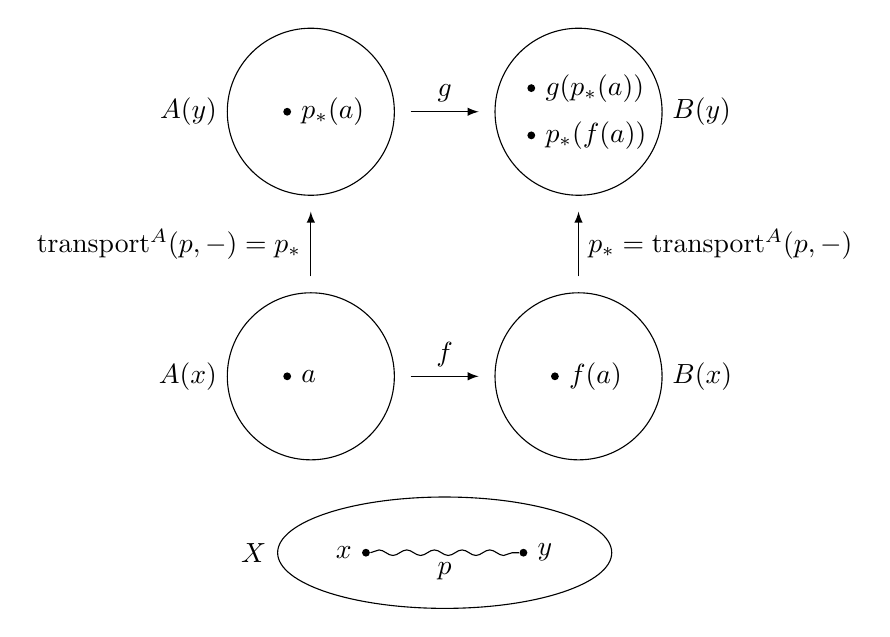
\begin{tikzpicture}[yscale=1,xscale=1]
  \def\xshift{1.7}
  \def\yheight{2.8}

  % A
  \node[circle,draw,inner sep=0.75cm,label=left:{$A(x)$}]
    (Ax) at (-\xshift,0.8*\yheight) {};
  \node[circle,draw,inner sep=0.75cm,label=left:{$A(y)$}]
    (Ay) at (-\xshift,2*\yheight) {};
  \node[circle,fill,inner sep=1pt,xshift=-0.3cm,label=right:{$a$}]
    (fa) at (Ax) {};
  \node[circle,fill,inner sep=1pt,xshift=-0.3cm,label=right:{$p_*(a)$}]
    (pa) at (Ay) {};

 % B
  \node[circle,draw,inner sep=0.75cm,label=right:{$B(x)$}]
    (Bx) at (\xshift,0.8*\yheight) {};
  \node[circle,draw,inner sep=0.75cm,label=right:{$B(y)$}]
    (By) at (\xshift,2*\yheight) {};
  \node[circle,fill,inner sep=1pt,xshift=-0.3cm,label=right:{$f(a)$}]
    (a) at (Bx) {};
  \node[circle,fill,inner sep=1pt,xshift=-0.6cm,yshift=0.3cm,label=right:{$g(p_*(a))$}]
    (gpa) at (By) {};
  \node[circle,fill,inner sep=1pt,xshift=-0.6cm,yshift=-0.3cm,label=right:{$p_*(f(a))$}]
    (pfa) at (By) {};


  \draw[->,shorten >=0.2cm,shorten <=0.2cm] (Ax) to[] node[auto] {$f$} (Bx) {};
  \draw[->,shorten >=0.2cm,shorten <=0.2cm] (Ay) to[] node[auto] {$g$} (By) {};
  \draw[->,shorten >=0.2cm,shorten <=0.2cm] (Ax) to[] node[auto] {$\operatorname{transport}^A(p,-)=p_*$} (Ay) {};
  \draw[->,shorten >=0.2cm,shorten <=0.2cm] (Bx) to[] node[auto, swap] {$p_*=\operatorname{transport}^A(p,-)$} (By) {};
  % % paths
  % \draw[->,shorten >=0.3cm,shorten <=0.3cm] (py) to[] node[auto] {$q_\ast$} (pz) {};
  % \draw[->,shorten >=0.3cm,shorten <=0.3cm, transform canvas={yshift=0.1cm}] (px) -- node[auto] {$q_\ast\circ p_\ast$} (pz) {};
  % \draw[->,shorten >=0.3cm,shorten <=0.3cm, transform canvas={yshift=-0.1cm}] (px) -- node[below] {$(p\ct q)_\ast$} (pz) {};
 

  % Base space X
  \node[circle,draw,inner sep=0.5cm,label=left:{$X$},xscale=3.0,yscale=1.0] (A) at (0,0) {};
  \node[circle,fill,inner sep=1pt,label=left:{$x$}] (x) at (-1.0,0) {};
  \node[circle,fill,inner sep=1pt,label=right:{$y$}] (y) at (1.0,0) {};
  \draw[decorate,decoration={snake,amplitude=1}] (x) -- node[auto,swap] {$p$} (y);
\end{tikzpicture}
\end{document}